\documentclass{beamer}
%%%%%%%%%%%%%%%%%%%%%%
% basic tutorial in german: http://www2.informatik.hu-berlin.de/~mischulz/beamer.html
%%%%%%%%%%%%%%%%%%%%%%

%------- packages ---------%
\usepackage[english]{babel}         %Umlaute, neue deutsche Rechtschreibung
\usepackage[utf8x]{inputenc}        %Kodierung festlegen, für UTF-8 Unterstützung entsprechend 
\usepackage{amsmath,amsfonts,amssymb}   %math. Symbole und Umgebungen
\usepackage{graphicx}
%\usepackage{natbib}

%------- theme and style ---------%
\usetheme{Boadilla}  %% Themenwahl
\usecolortheme{default}
\usefonttheme{default}
\useinnertheme{circles}     %	{circles | default | inmargin |	rectangles | rounded}
\useoutertheme{default} %	default | infolines | miniframes | shadow | sidebar | smoothbars |smoothtree | split | tree}
%\beamertemplatenavigationsymbolsempty   % disable navigation simbols
%\bibliographystyle{apalike}
%------- metainformation ---------%

\title[Elementary flux mode analysis]{Designing optimal cell factories: integer programming couples elementary mode analysis with regulation\\~\\}
\subtitle{Molecular Networks B SS13}
\author[Jonas Ibn-Salem]{Jonas Ibn-Salem}
\institute[]{}
\date{25.04.13}
%\logo{\pgfimage[width=2cm,height=0.5cm]{grafik/FULogo_RGB}}
\titlegraphic{
\includegraphics[width=4cm,height=1cm]{grafik/FULogo_RGB}}


\begin{document}
%\frame{\titlepage}
\maketitle

% OUTLINE:
%- Metabolically engineering: 
%  - strain improvement 
%  - efficient deletion strategies
% -steady state assumption, 
% -elementary mode (EM)
% -constrained minimal cut sets
% -network of minimal functionality
% -advantage of inclusion of regulatory information
%%%%%%%%%%%%%%%%%%%%%%%%%%%%%%%%%%%%%%%%%%%%%%%%%%%%%%%%%%%%%%%%%%%%%%%% 
% Preface stuff:
%%%%%%%%%%%%%%%%%%%%%%%%%%%%%%%%%%%%%%%%%%%%%%%%%%%%%%%%%%%%%%%%%%%%%%%% 

\begin{frame}{Overview}
    \tableofcontents
\end{frame}

%%%%%%%%%%%%%%%%%%%%%%%%%%%%%%%%%%%%%%%%%%%%%%%%%%%%%%%%%%%%%%%%%%%%%%%% 
\section{Introduction and Repetition}
%%%%%%%%%%%%%%%%%%%%%%%%%%%%%%%%%%%%%%%%%%%%%%%%%%%%%%%%%%%%%%%%%%%%%%%% 

\begin{frame}{Metabolic network}
    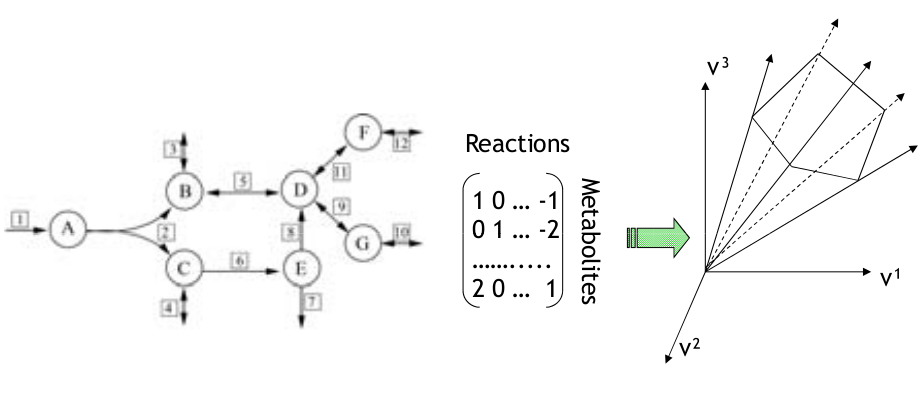
\includegraphics[width=\textwidth]{grafik/modelling} \\
    \footnotesize{
        source A.Bockmayer lecture slides Algorithms in Systembiology SS12
        }
    \begin{columns}
    \column{.7\textwidth}    
        Model of metabolic network with
        \begin{itemize}
            \item $m$ internal metabolites
            \item $n$ reactions
            \item $S \in \mathbb{R}^{m\times n}$ stoichiometric matrix
            \item $\hat{v} \in \mathbb{R}^{n}$ flux vector
        \end{itemize}
    \column{.3\textwidth}    
        fig?
    \end{columns}
\end{frame}

\begin{frame}{Steady state assumption}    
    \begin{block}{Steady state assumption}
        Metabolite concentrations and reaction rates are constant.
    \end{block}
    \begin{equation}
    %\Rightarrow 
    S \cdot \hat{v} = 0 
    \end{equation}
    Steady state flux coen: \\
    $C = \{v \in \mathbb{R}^n | Sv = 0, v_i \geq 0, i \in Irr \}$
\end{frame}

\begin{frame}{Elementary mode analysis}
    \begin{itemize}
        \item For $v \in \mathbb{R}^n$, the support of v is defined as 
        $supp(v) = \{i \in \{1, ..., n \} | v_i \neq 0  \}$
    
        \item $v \in C$ is an \emph{elementary flux mode} if $supp(v)$
        is minimla w.r.t $\subseteq$
        i.e, if there is no $v' \in C, v' \neq 0$ with 
        $supp(v') \subsetneq supp(v)$.
    \end{itemize}
    
    
    \begin{definition}
        An elementary mode (EM) is a minimal and indivisible set 
        of reactions that operates under steady state conditions, 
        while obeying all (ir-)reversibility constraints.
    \end{definition}
    
\end{frame}
\begin{frame}{Elementary mode example}
    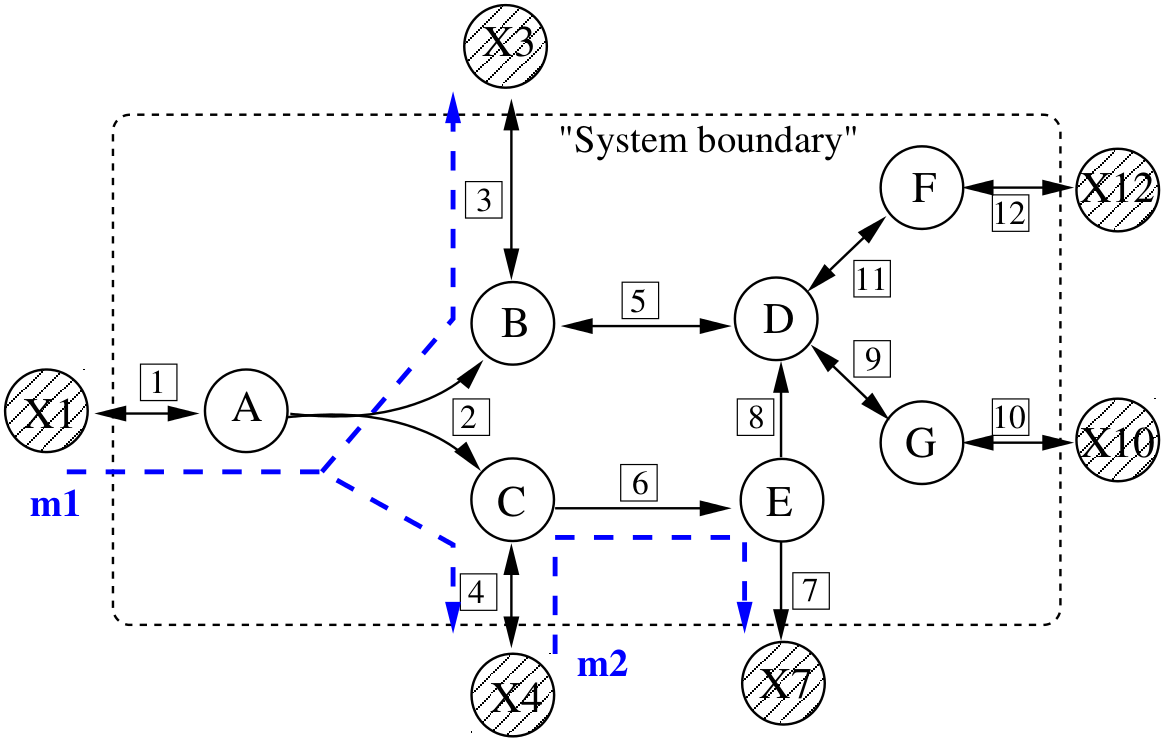
\includegraphics[width=.7\textwidth]{grafik/EMnet1}
    \begin{itemize}
        \item $m^{1} = (1, 1, 1, 1, 0, 0, 0, 0, 0, 0, 0 ,0)$
        \item $m^{1} = (0, 0, 0, -1, 0, 1, 1, 0, 0, 0, 0 ,0)$
        \item $m^{1}$ and $m^{2}$ are elementary modes.
    \end{itemize}
\end{frame}

\begin{frame}{Elementary mode example (ctd)}
    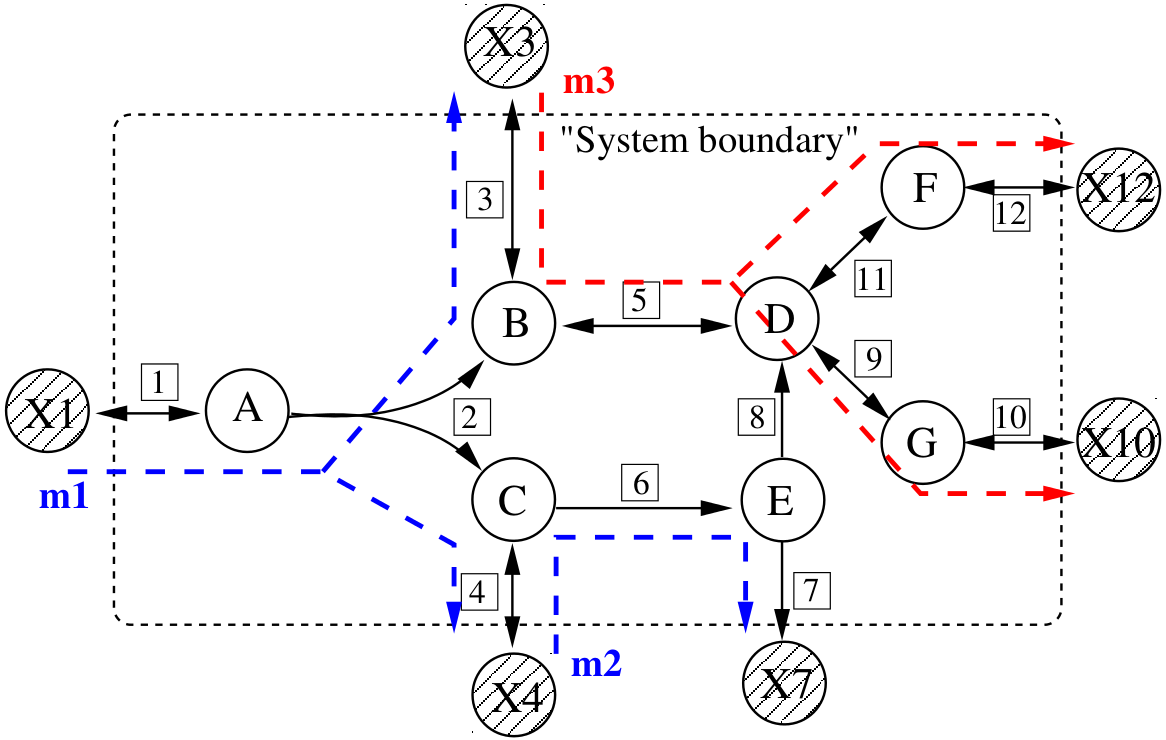
\includegraphics[width=.7\textwidth]{grafik/EMnet2}
    \begin{itemize}
        \item $m^{3} = (0, 0, 2, 0, 2, 0, 0, 0, 1, 1, 1 ,1)$
        \item $m^{3} = m^{4} + m^{5}$, with
        \begin{itemize}
            \item $ m^{4} = (0, 0, 1, 0, 1, 0, 0, 0, 1, 1, 0 ,0)$
            \item $ m^{5} = (0, 0, 1, 0, 1, 0, 0, 0, 0, 0, 1 ,1)$
        \end{itemize}
        \item Since $m^{4}, m^{5} \in C, supp(m^{4}), supp(m^{5}) \subsetneq supp(m^{3})$, $m^{3}$ is not an elementary flux mode.
    \end{itemize}
\end{frame}

%%%%%%%%%%%%%%%%%%%%%%%%%%%%%%%%%%%%%%%%%%%%%%%%%%%%%%%%%%%%%%%%%%%%%%%% 
\section{Motivation and Theory}
%%%%%%%%%%%%%%%%%%%%%%%%%%%%%%%%%%%%%%%%%%%%%%%%%%%%%%%%%%%%%%%%%%%%%%%% 

\begin{frame}{Paper and authors}
    
\includegraphics[width=1\textwidth]{grafik/paper}
    \begin{columns}
    \column{.3\textwidth}
      \begin{center}
        \begin{figure}
         
\includegraphics[width=0.5\textwidth]{grafik/jungreuthmayer} \\
         \tiny{source: biotec.boku.ac.at}
        \end{figure}
      \end{center}
    \column{.3\textwidth}
      \begin{center}
        \begin{figure}
         
\includegraphics[width=0.5\textwidth]{grafik/zanghellini} \\
         \tiny{source: biotec.boku.ac.at}
        \end{figure}
      \end{center}
    \column{.3\textwidth}
    \tiny {$^{1}$ Austrian Centre of Industrial 
        Biotechnology, Vienna, Austria} 
    \\ ~ \\
    \tiny {$^{2}$ Department of Biotechnology, 
        University of Natural Resources and Life Sciences, 
        Vienna, Austria} 
 \end{columns}
\end{frame}

\begin{frame}{Background and Motivation}
    \begin{itemize}
        \item microbes can be used for metabolic engineering 
        e.g. ethanol production in \emph{E. coli}
        \item Methabolic networks are available for some model organisms
    \end{itemize}
    \begin{block}{Gaol}
        Gene deletion strategie to optimize the production 
        efficiency of strains.
    \end{block}
\end{frame}


\begin{frame}{Network of minimal functionality (NMF)}
    
\end{frame}

\begin{frame}{Theory: Elementary mode analysis}
    $e = e(\hat{e}) $ is the binary representation of a EM $e$.
    \begin{equation}
        e_{i} := e(\hat{e}_{i})) = 
        \begin{cases}
            1 & \text{if }  \hat{e}_{i} \neq 0 \\
            0 & \text{if }  \hat{e}_{i} = 0 
        \end{cases}
    \end{equation}
    $ e^{T}v \leq e^{T}e = \sum_{i=1}^{n} e_{i}^{2} = \sum_{i=1}^{n} e_{i} =: ||e||$

\end{frame}

\begin{frame}{Binary linear program (BLP)}
    Group all $q$ elementary modes:
    \begin{align*}
        G &:= (e_{1}, ..., e_{r})^{T}            &\text{\emph{goal matrix} with desirable EM}   &\\
        H &:= (e_{r+1}, ..., e_{r+s})^{T}        &\text{\emph{helper matrix} tolerated EM}      &\\
        K &:= (e_{r+s+1}, ..., e_{r+s+t})^{T}    &\text{\emph{kill matrix} unwanted EM}         &\\
    \end{align*}
where $q = r+s+t$
\end{frame}

\begin{frame}{Binary linear program (BLP)}
    
$max ~||x||$ \\
s.t. 
\begin{align*}
    e^{T}_{g} x & =       ||e_{g}||      & g \in \{1, ..., r\}     &~\\
    e^{T}_{h} x & \leq    ||e_{h}||     & h \in \{r+1, ..., r+s\} &~\\
    e^{T}_{k} x & \leq    ||e_{k}||-1  & k \in \{r+s+1, ..., r+s+t\} &~\\
\end{align*}
$x = (x_{1}, ..., x_{n})^{T}, \quad x_{i} \in \{0, 1\} \forall i$
%where
%\begin{align*}
%    |g| &= (||e_1||, ..., ||e_r||)^T \\
%    |h| &= (||e_{r+1}||, ..., ||e_{r+s}||)^T \\
%    |k| &= (||e_{r+s+1}||, ..., ||e_{r+s+t}||)^T \\
%\end{align*}

\begin{align*}
    \Delta_{min} = n - ||x||
\end{align*}

\end{frame}

\begin{frame}{Alternative solutions}
\begin{itemize}
    \item The BLP may have no or a finite number of solutions.
    \item Iteratively exclude existing solutions $x^{(j)}$ by adding constraints:
\end{itemize}
    
    \begin{align*}
        \sum_{i \in B} x_i & \leq |B| -1 \\
        \sum_{i \in N} x_i & \geq 1   \\
    \end{align*}
    where 
    \begin{align*}
        B = \{i |x_{i}^{(j)} = 1\} \\
        N = \{i |x_{i}^{(j)} = 0\} \\
    \end{align*}

\end{frame}


%%%%%%%%%%%%%%%%%%%%%%%%%%%%%%%%%%%%%%%%%%%%%%%%%%%%%%%%%%%%%%%%%%%%%%%% 
\section{Illustrative example}
%%%%%%%%%%%%%%%%%%%%%%%%%%%%%%%%%%%%%%%%%%%%%%%%%%%%%%%%%%%%%%%%%%%%%%%% 
\begin{frame}{Illustrative example}
    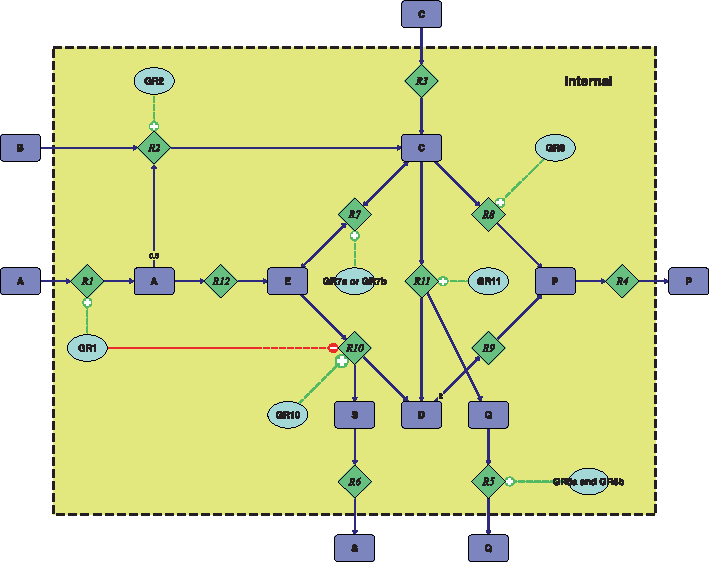
\includegraphics[width=.9\textwidth]{grafik/fig1} \\
\end{frame}


\begin{frame}{Elementary modes}
    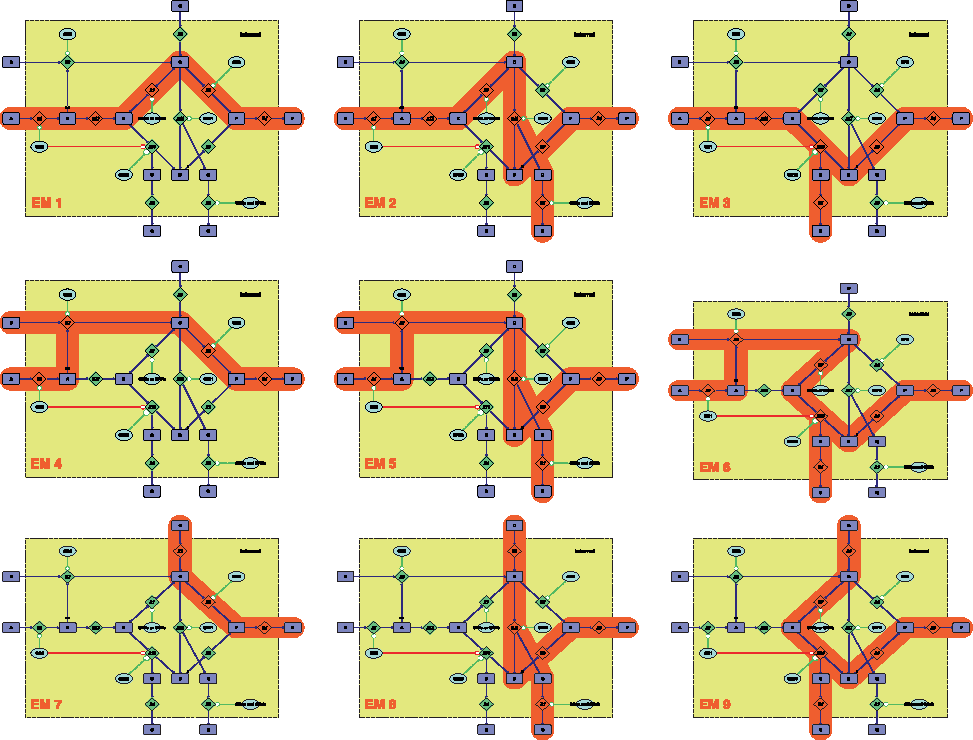
\includegraphics[width=.9\textwidth]{grafik/fig2} \\
\end{frame}

\begin{frame}{List of elementary modes}
    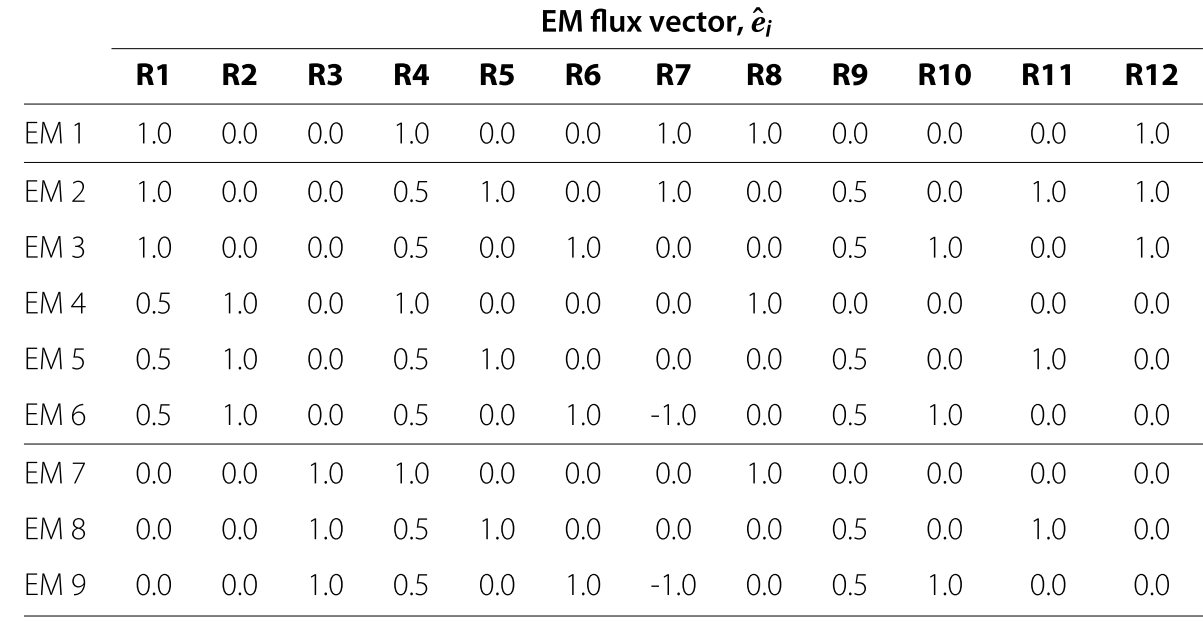
\includegraphics[width=\textwidth]{grafik/table1a} \\
\end{frame}

\begin{frame}{List of binary elementary modes}
    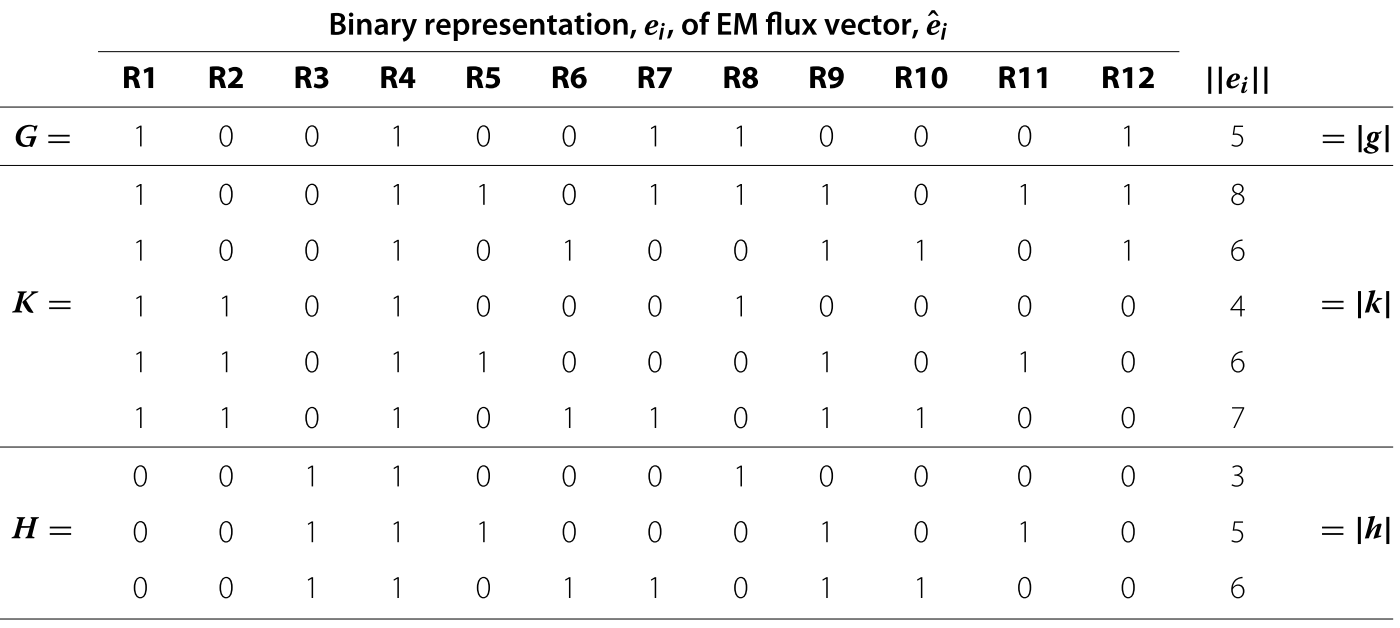
\includegraphics[width=\textwidth]{grafik/table1b} \\
\end{frame}

\begin{frame}{BLP for example network}
    $$max \sum_{i=1}^{12} x_i$$
     
    \begin{align*}
\text{subject to}\quad\quad\quad\quad
    x_1 + x_4 + x_7 + x_8 + x_{12}                      & = 5   \\
    \\
    x_3 + x_4 + x_8                                     & \leq 3 \\
    x_3 + x_4 + x_5 + x_9 + x_{11}                      & \leq 5 \\
    x_3 + x_4 + x_6 + x_7 + x_9 + x_{10}                & \leq 6 \\
    x_1 + x_4 + x_5 + x_7 + x_8 + x_9 + x_{11} + x_{12} & \leq 7 \\
    x_1 + x_4 + x_6 + x_9 + x_{10} + x_{12}             & \leq 5 \\
    \\
    x_1 + x_2 + x_4 + x_8                               & \leq 3 \\
    x_1 + x_2 + x_4 + x_5 + x_9 + x_{11}                & \leq 5 \\
    x_1 + x_2 + x_4 + x_6 + x_7 + x_9 + x_{10}          & \leq 6 \\
    \end{align*}
\end{frame}


\begin{frame}{Minimal cut sets}
    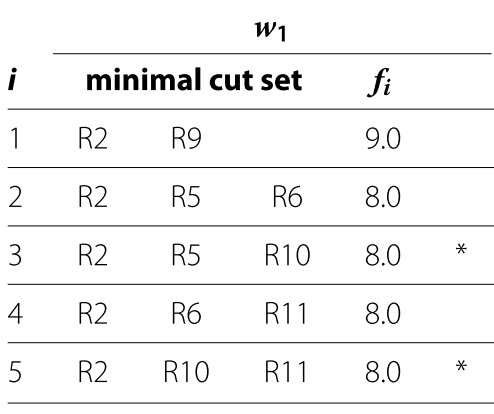
\includegraphics[height=5cm]{grafik/table2a} \\
\end{frame}

\begin{frame}{Biological feasibility}
    Problem:
    \begin{itemize}
        \item Distinguish chemical from genetic interventions
        \item Gene-enzyme-reaction mapping not always known.
    \end{itemize}
    Solution: 
    \begin{itemize}
        \item add weights to objective function
        $$max ||w^T x|| $$
        \item low weights for uptake reactions
        \item high weights for reactions with missing genetic information
    \end{itemize}
    \begin{example}
        $$w_2^T = (0.1, ~ 0.1, ~ 0.1, ~ 99, ~ 1, ~ 99, ~ 2, ~ 1, ~ 99, ~ 1, ~ 1, ~ 99)$$
    \end{example}
\end{frame}

\begin{frame}{Minimal cut sets wights wights}
    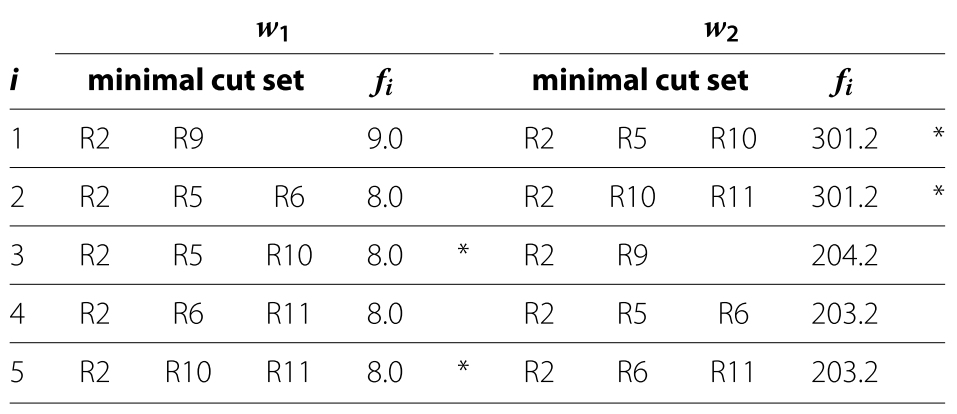
\includegraphics[height=5cm]{grafik/table2} \\
\end{frame}


%%%%%%%%%%%%%%%%%%%%%%%%%%%%%%%%%%%%%%%%%%%%%%%%%%%%%%%%%%%%%%%%%%%%%%%% 
\section{Including regulation and optimizing metabolic functionality}
%%%%%%%%%%%%%%%%%%%%%%%%%%%%%%%%%%%%%%%%%%%%%%%%%%%%%%%%%%%%%%%%%%%%%%%% 


%%%%%%%%%%%%%%%%%%%%%%%%%%%%%%%%%%%%%%%%%%%%%%%%%%%%%%%%%%%%%%%%%%%%%%%% 
\section{Realistic example: Ethanol production in E. coli}
%%%%%%%%%%%%%%%%%%%%%%%%%%%%%%%%%%%%%%%%%%%%%%%%%%%%%%%%%%%%%%%%%%%%%%%% 

%%%%%%%%%%%%%%%%%%%%%%%%%%%%%%%%%%%%%%%%%%%%%%%%%%%%%%%%%%%%%%%%%%%%%%%% 
\section{Summary and conclusions}
%%%%%%%%%%%%%%%%%%%%%%%%%%%%%%%%%%%%%%%%%%%%%%%%%%%%%%%%%%%%%%%%%%%%%%%% 

%%%%%%%%%%%%%%%%%%%%%%%%%%%%%%%%%%%%%%%%%%%%%%%%%%%%%%%%%%%%%%%%%%%%%%%% 
%%%%%%%%%%%%%%%%%%%%%%%%%%%%%%%%%%%%%%%%%%%%%%%%%%%%%%%%%%%%%%%%%%%%%%%% 
\begin{frame}{Introduction: Fixed Point Analysis}
    Given the system of differential equations:
    $$y' = f(y) $$
    \begin{definition}
        A \emph{fixed point $y^*$} is defined by $f(y^*)=0$.
    \end{definition}
    %$\Rightarrow$ 
    \begin{itemize}
        \item Solve the equation $f(y) = 0$ 
        \item Analyse eigenvalues of the Jacobian at fixed points.
    \end{itemize}
    Now: System with \emph{controle parameter} $\mu$. 
    $$y' = f(y, \mu)$${}    
    \begin{block}{}
        How does $\mu$ influence the number, location and stability of fixed points?
    \end{block}
\end{frame}

\end{document}
%%%%%%%%%%%%%%%%%%%%%%%%%%%%%%%%%%%%%%%%%%%%%%%%%%%%%%%%%%%%%%%%%%%%%%%% 
% Stuff:
%%%%%%%%%%%%%%%%%%%%%%%%%%%%%%%%%%%%%%%%%%%%%%%%%%%%%%%%%%%%%%%%%%%%%%%% 

%TODO:
%    - irreversable reactions in model
%   - constraints for binary variables in IP 
